\newcommand{\ConstExercise}{2}
\newcommand{\ConstDeadline}{21.04.2023}

\documentclass[11pt,letterpaper]{article}
\textwidth 6.5in
\textheight 9.in
\oddsidemargin 0in
\headheight 0in

\usepackage[dark,exp]{custom_0.1}

\begin{document}

%%%%% Document %%%%%
\begin{enumerate}
  \item \textbf{Wärmeleitung I}
    \begin{enumerate}
      \item
        \begin{align*}
          \vec{j}_Q &= -\lambda\cdot \vec{\nabla}T\\
          j_Q&= \lambda \frac{\abs{\Delta T}}{d}\\
          \\
          &= 0.8\,\ufrac{W}{mK} \frac{40\,^\circ\mathrm{K}}{5\cdot 10^{-3}\, \mathrm{m}}\\
          &= 6400\,\ufrac{W}{m^2}
        \end{align*}

      \item
        Die Temperatur der äußeren Seite der inneren Scheibe ist gleich der Innentemperatur,
        analog dazu ist die Temperatur der äußere Seite der äußeren Scheibe gleich der Außentemperatur.
        Dies liegt daran das der der Temperaturverlauf stetig ist, und der Formel nach ein 
        abrupter Temperaturwechsel zu einer unendliche Wärmestromdichte führen würde:
        \begin{align*}
          \lim_{d\to 0}j_Q &= \lim_{d\to 0}\lambda \frac{\abs{\Delta T}}{d} = \infty \quad \text{, für } \Delta T >0
        \end{align*}

      \item
        \begin{align*}
          j_Q&= \lambda \frac{\abs{\Delta T}}{d}\\
          \Delta T_{i} &= \frac{j_Q d_i}{\lambda_i}\\
          \sum_{i} \Delta T_{i} &= \abs{T_1 - T_2} = j_Q \sum_i \frac{ d_i}{\lambda_i}\\
          j_Q &= \frac{\Delta T}{ \sum_i \frac{ d_i}{\lambda_i}}\\
          \\
        \end{align*}
    \end{enumerate}

  \item \textbf{Spezifische Wärme}
    \begin{align*}
      E_{th} &= E'_{th}\\
      T_1 \cbrace{c_{\ch{H2O}}m_{\ch{H2O}} + c_{\ch{Cu}} m_{\ch{Cu},1}} + T_2 c_{\ch{Cu}} m_{\ch{Cu},2}&= 
      T_3 \cbrace{c_{\ch{H2O}}m_{\ch{H2O}} + c_{\ch{Cu}} (m_{\ch{Cu},1} + m_{\ch{Cu},2})}\\
      c_{\ch{H2O}}m_{\ch{H2O}} \cbrace{T_1 - T_3}&= 
      c_{\ch{Cu}} (T_3 (m_{\ch{Cu},1} + m_{\ch{Cu},2})- T_1 m_{\ch{Cu},1} - T_2 m_{\ch{Cu},2} )\\
      c_{\ch{Cu}}  &= \frac{c_{\ch{H2O}}m_{\ch{H2O}} \cbrace{T_1 - T_3}}{ T_3 (m_{\ch{Cu},1} + m_{\ch{Cu},2}) - T_1 m_{\ch{Cu},1} - T_2 m_{\ch{Cu},2} }\\
      &= \frac{c_{\ch{H2O}}m_{\ch{H2O}} \cbrace{T_1 - T_3}}
      {  m_{\ch{Cu},1}(T_3-T_1) + m_{\ch{Cu},2}(T_3-T_2) }\\
      &= -\frac{c_{\ch{H2O}}m_{\ch{H2O}} }
      {  m_{\ch{Cu},1} + m_{\ch{Cu},2}\frac{T_3-T_2}{T_3-T_1} }\\
      \\
      &= - \frac{4190 \,\ufrac{J}{kg\,K}\cdot 0.3\,\mathrm{kg}}{0.187\,\mathrm{kg} 
      + 0.089\,\mathrm{kg} \frac{20.2\,\mathrm{K}-97.8\,\mathrm{K}}{20.2\,\mathrm{K}-18.2\,\mathrm{K}}}\\
      &\approx 384\,\ufrac{J}{kg\,K}
    \end{align*}


  \item \textbf{Thermische Eigenschaften von Stickstoff}
    \begin{enumerate}
      \item
        \begin{align*}
          \braket{E_{kin}}&= \frac{3}{2}k_B T\\
          &\approx \frac{3}{2} \cdot 1.381\cdot 10^{-23}\,\ufrac{J}{K} 273\,\mathrm{K}\\
          &\approx 5.66  \cdot 10^{-21}\,\mathrm{J}
        \end{align*}

      \item
        \begin{align*}
          \braket{E_{kin}} &= \frac{1}{2}m\braket{v^2}\\
          \sqrt{\braket{v^2}} &= \sqrt{\frac{2 \braket{E_{kin}}}{m}}\\
          &\approx \sqrt{\frac{2 \cdot  5.66  \cdot 10^{-21}\,\mathrm{J}}{2\cdot 0.014\ufrac{kg}{mol} \cdot (6.022\cdot 10^{23} \,\ufrac{1}{mol})^{-1}}}\\
          &\approx 493\,\ufrac{m}{s}
        \end{align*}

      \item \, \\
      \begin{figure*}[]
        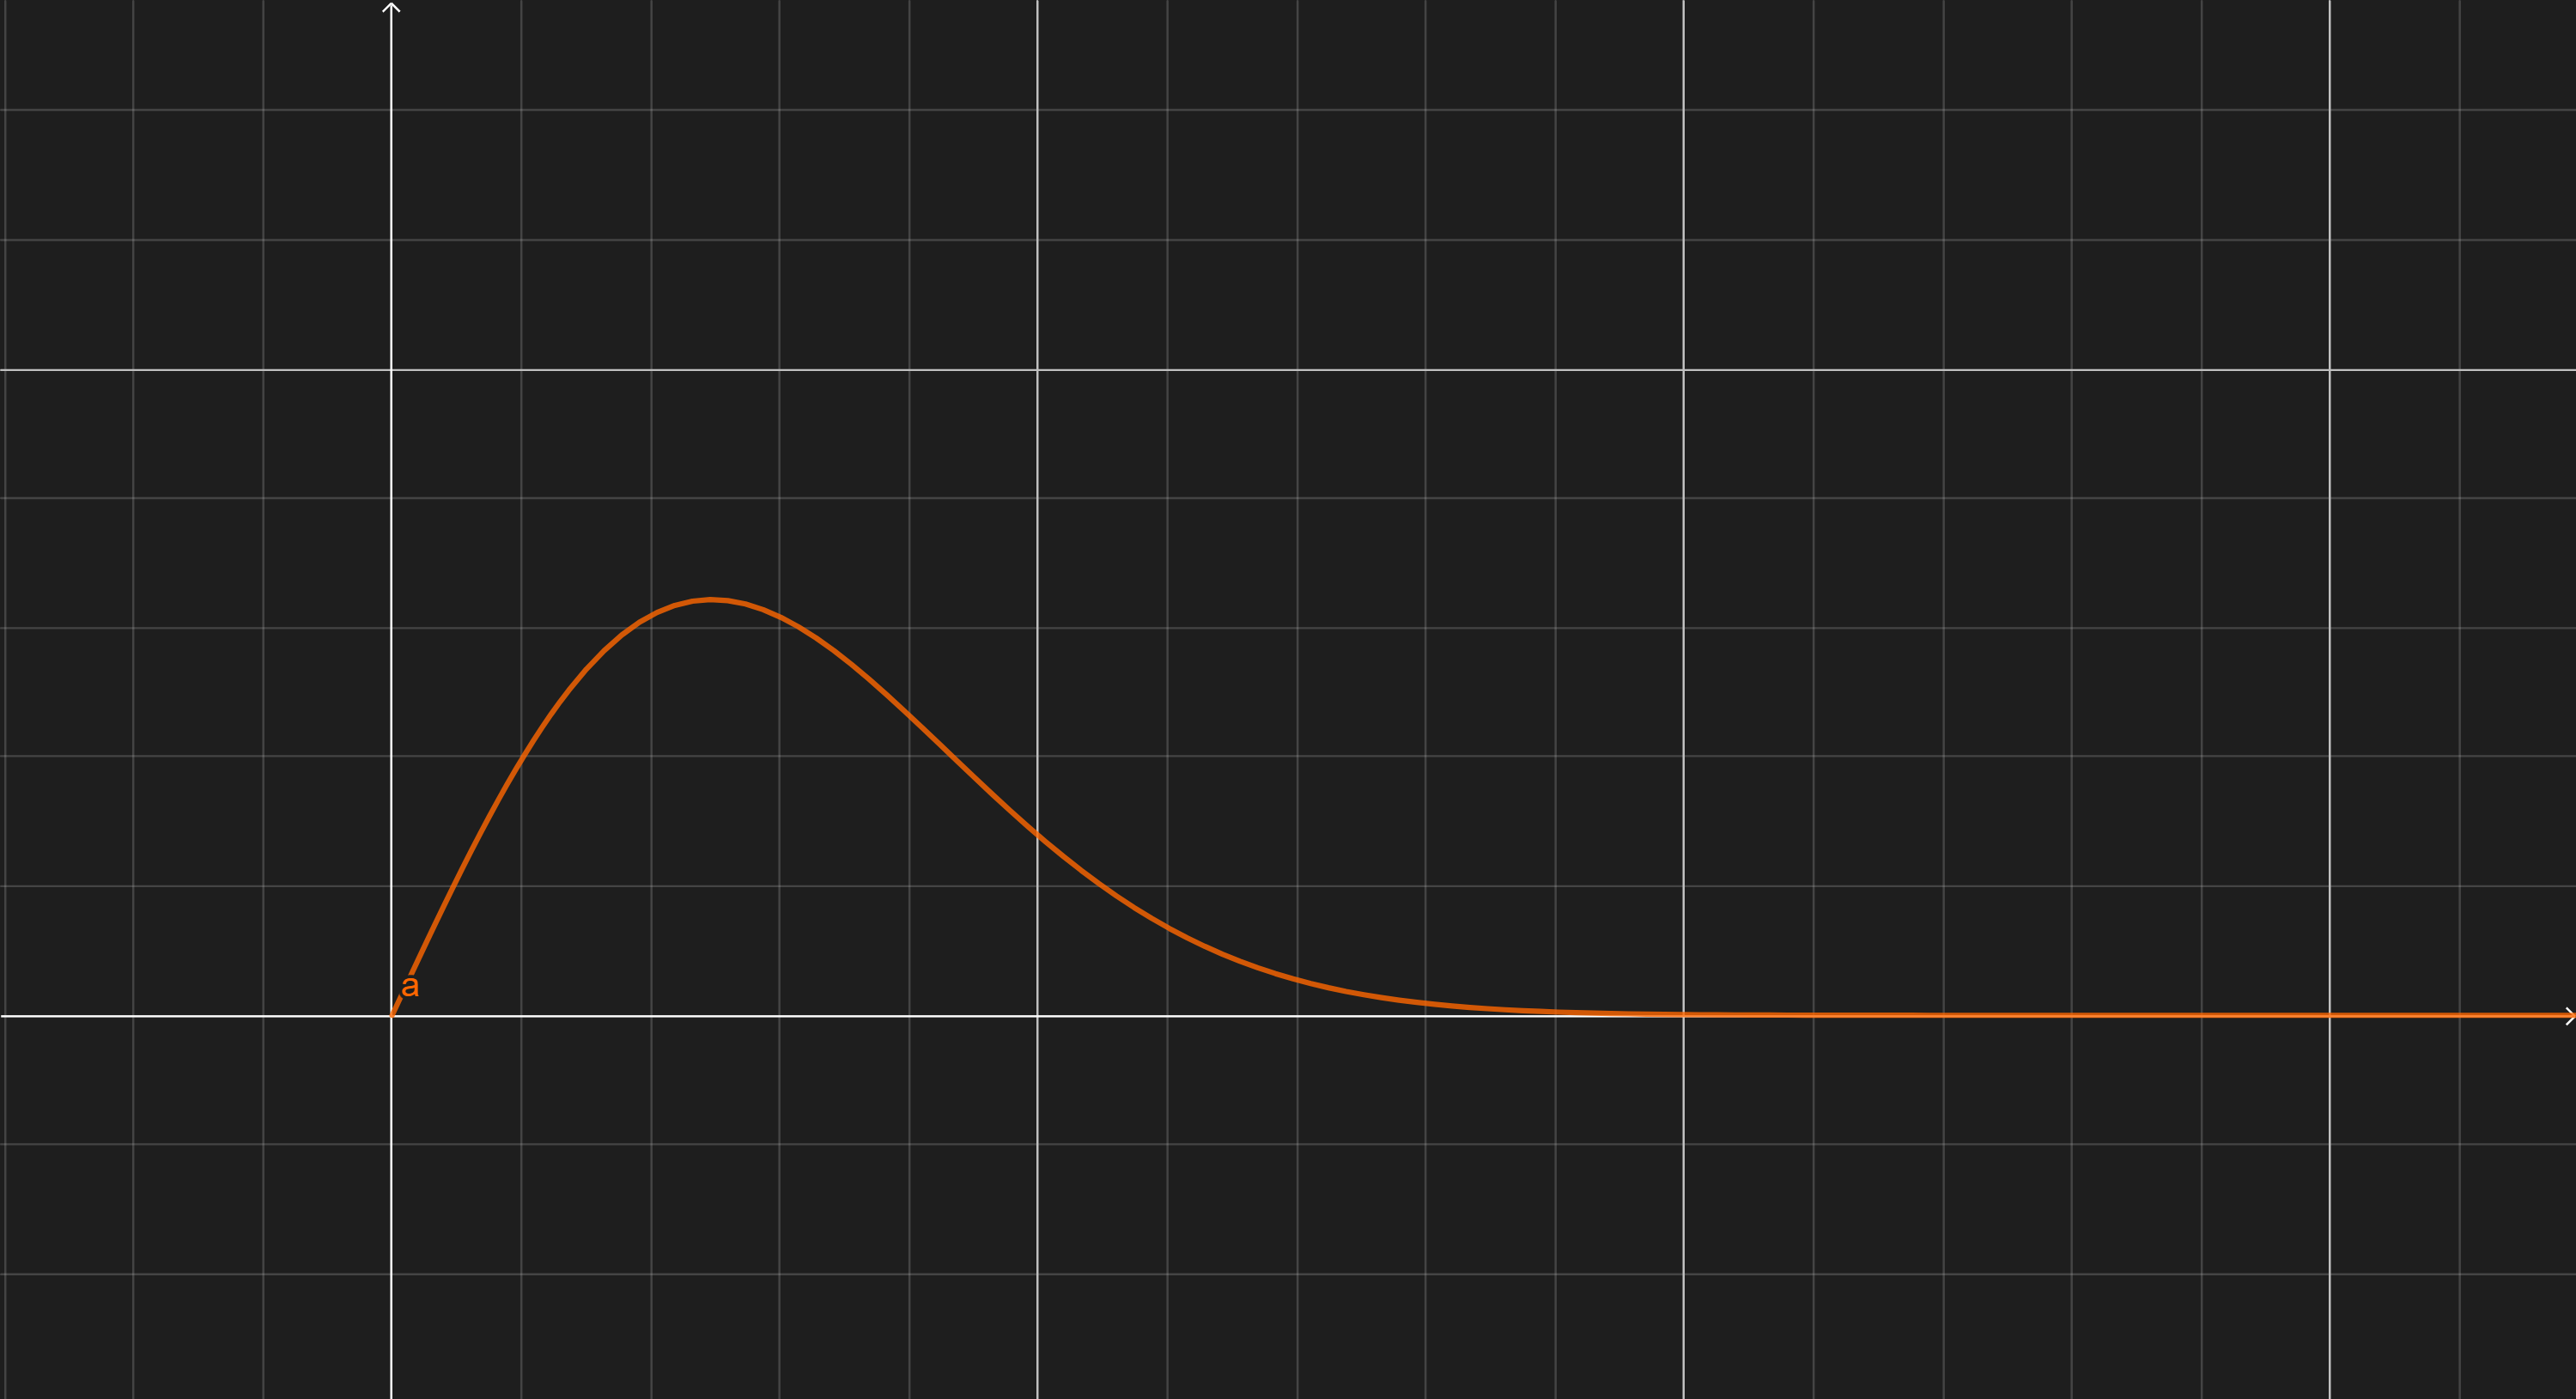
\includegraphics[width = 0.8 \textwidth]{1.png}
        \caption{Boltzmann-Verteilung}
        \centering
      \end{figure*}
      
        \begin{align*}
          v_w < \mu(f(v_w)) \le \sqrt{\braket{v^2}}
        \end{align*}

      \item
        \begin{align*}
          \rho &= \frac{m}{V}\\
          \\
          pV &= Nk_B T\\
          V &= \frac{Nk_BT}{p}\\
          \\
          \rho &= \frac{mp}{Nk_BT}\\
          &\approx \frac{0.028\,\mathrm{kg}\cdot 1.01\cdot 10^{5}\,\mathrm{Pa}}
          {6.022\cdot 10^{23} \cdot 1.381\cdot 10^{-23}\,\ufrac{J}{K} \cdot 273\,\mathrm{K}}\\
          &\approx 1.25 \,\frac{kg}{m^3} 
        \end{align*}

      \item 
        \begin{align*}
          \braket{F} &= \braket{\Delta p} \cdot f\\
          &= m\braket{\Delta v} \cdot \frac{\braket{v}}{d}\\
          &= 2m\braket{v} \cdot \frac{\braket{v}}{V^{\frac{1}{3}}}\\
          &= 2m \braket{v}^2\cbrace{\frac{p}{Nk_BT}}^{\frac{1}{3}}\\
          &= 4\braket{E_{kin}}\cbrace{\frac{p}{Nk_BT}}^{\frac{1}{3}}\\
          &= 6 k_B T \cbrace{\frac{p}{Nk_BT}}^{\frac{1}{3}}\\
          &= 6 \cbrace{k_B T}^{\frac{2}{3}} \cbrace{\frac{p}{N}}^{\frac{1}{3}}\\
          &\approx 6 \left(\kb \cdot 273\,\mathrm{K}\right)^{\frac{2}{3}}\cbrace{\frac{1.01\cdot 10^5\,\mathrm{Pa}}{\na}}^{\frac{1}{3}}\\
          &\approx 8.01 \cdot 10^{-20}\mathrm{N}
        \end{align*}
        \begin{align*}
          {p} &= \frac{F}{A} 
          = \frac{N \braket{F}}{6\cdot d^2}\\
          &= \frac{N \cdot 6 \cbrace{k_B T}^{\frac{2}{3}} \cbrace{\frac{p}{N}}^{\frac{1}{3}}}{6\cdot d^2}\\
          &= \frac{ \cbrace{N k_B T}^{\frac{2}{3}} {p}^{\frac{1}{3}}}{ \cbrace{\frac{Nk_BT}{p}}^{\frac{2}{3}}}\\
          &= p \qquad \qquad \text{:D}\\
        \end{align*}
    \end{enumerate}

\newpage
  \item \textbf{Um welches Gas handelt es sich? }
    \begin{enumerate}
      \item
        \begin{align*}
          \braket{E_{kin}} &= \frac{\braket{p^2}}{2m}\\
          m  &= \frac{\braket{p^2}}{2 \braket{E_{kin}}}\\
          &= \frac{8.18\cdot 10^{-46}\,\frac{kg^2m^2}{s^2}}{2 \cdot 6.17\cdot 10^{-21}\,\mathrm{J}}\\
          &\approx 6.63 \cdot 10^{-26}\,\mathrm{kg} \\
          &\approx 40\,\ufrac{g}{mol}
        \end{align*}
        Mögliche Gase sind: Argon, Cyclopropen, Propadien, Propin und weitere\\

      \item
        Die gesamte innere Energie zu kennen, würde dabei helfen Moleküle nicht nur anhand
        ihrer Masse unterscheiden zu können, sondern auch mittels ihres molekularen Aufbaus/Freiheitsgrade. 
        So könnte man z.B. die oben genannten Gase auseinander halten, und das obwohl alle 
        außer Argon sich die identische Strukturformel teilen.
    \end{enumerate}

  \item \textbf{Steigende Luftblase}
    \begin{enumerate}
      \item
        \begin{align*}
          p_{extern} &=  p_{intern}\\
          \rho_w g h + p_{atmos} &=  \frac{Nk_BT}{V}\\
          N &= V\frac{\rho_w g h + p_{atmos}}{k_B T}\\
          V' &= \frac{N k_B T'}{\rho_w g h' + p_{atmos}}\\
          &= \frac{V\frac{\rho_w g h + p_{atmos}}{k_B T} k_B T'}{\rho_w g h' + p_{atmos}}\\
          &\overset{h'=0}{=} V \frac{T'}{ T} \left(\frac{\rho_w g h}{ p_{atmos}} +1 \right)\\
          &\approx 10\,\mathrm{cm^3} \frac{277.15\,\Kelvin}{298.15\Kelvin}
          \cbrace{ \frac{10^3 \,\ufrac{kg}{m^3} \, \cdot 9.81\,\ufrac{m}{s^2} \cdot 60\,\mathrm{m}}
          {1.01\cdot 10^5 \,\mathrm{Pa}} +1 } \\
          &= 6.35\,\mathrm{cm}^3\\
        \end{align*}

      \item
        \begin{align*}
          F_\sigma &= F_{extern}\\
          \Delta E_{\sigma} &= \Delta E_{extern}\\
          \\
          2\varepsilon \Delta A &= \Delta p A \Delta r \\
          2\varepsilon \cdot 4\pi((r+\Delta r)^2-r^2) &= \Delta p\cdot 4\pi r^2 \cdot \Delta r \\
          \Delta p &= 2\varepsilon \frac{(r+\Delta r)^2-r^2}{ r^2 \Delta r} \\
          &= 2\varepsilon \frac{r^2+2r\Delta r+\Delta r^2-r^2}{ r^2 \Delta r} \\
          &= 2\varepsilon \frac{2r\Delta r+\Delta r^2}{ r^2 \Delta r} \\
          &= 4\frac{\varepsilon}{r} +2\Delta r \frac{\varepsilon}{r^2}\\
          &= 4\frac{\varepsilon}{r} = 4\frac{\sigma}{r} \\
          \\
          \frac{\Delta p}{p_{extern}} &= \frac{4\frac{\sigma}{r}}{\rho_w g h + p_{atmos}}\\
          &= \frac{4\sigma\cbrace{\frac{3}{4 \pi}V}^{-\frac{1}{3}}}{\rho_w g h + p_{atmos}}\\
          \\
          \frac{\Delta p}{p_{extern}}(-60\,\mathrm{m}) &= 6.82\cdot 10^{-12} \approx 0\\
          \frac{\Delta p}{p_{extern}}(0\,\mathrm{m}) &= 4.70\cdot 10^{-11} \approx 0\\
        \end{align*}
    \end{enumerate}

\end{enumerate}

\end{document}